% ============================================================
%  NEUTRONICS ANALYSES
% ============================================================

Neutronics analyses were performed using the Serpent~2 Monte Carlo neutron and photon transport code \cite{Leppanen2025Status2024}. Serpent was selected over deterministic alternatives for its advanced capabilities in coupled burnup calculations, including: burnup-dependent geometry evolution, detailed chemical and radiological toxicity tracking, flexible depletion zone subdivision, universe nesting and reflective symmetry options, efficient parallel processing via domain decomposition, robust material definition transfers between models via binary restart files, fine control of numerical solvers (CRAM, TTA, and substep methods), and a comprehensive Python-based output-parsing library (SerpentTools) \cite{Johnson2020SerpentTools:Serpent}. These features are particularly well-suited to the multi-physics demands of the Lead-cooled Breeder Reactor (LBR) design workflow, where spent fuel material compositions must be reliably transported across successive simulation stages.

% ============================================================
\subsection{Spent Fuel Characterization: TMI-1 Benchmark}
% ============================================================

Spent fuel material definitions were generated using an axially-resolved model of a fuel assembly from Three Mile Island Unit~1 (TMI-1). TMI-1 was selected as the benchmark case due to the availability of well-documented, spatially resolved isotopic and burnup distribution data for the assembly NJ05YU, which enables rigorous verification and validation (V\&V) of the depletion methodology prior to application in the LBR design iteration \cite{Wolf2000AnalysisReport}. The Serpent model geometry was constructed on the basis of a 1998 MCNP reference calculation \cite{Wright1998CRCI.}.

The assembly geometry, shown in Figure~\ref{fig:tmi_geometry}, is discretized axially into a series of depletion zones to capture the spatially non-uniform burnup profile that results from flux gradients, control rod positioning, and coolant density variation along the rod length. Structural components — including upper and lower grid spacers, flanges, and flow distribution hardware — are explicitly modeled with region-specific material assignments. Key geometric and material parameters are summarized in Table~\ref{tab:figure_labels}.

\begin{figure}[H]
    \centering
    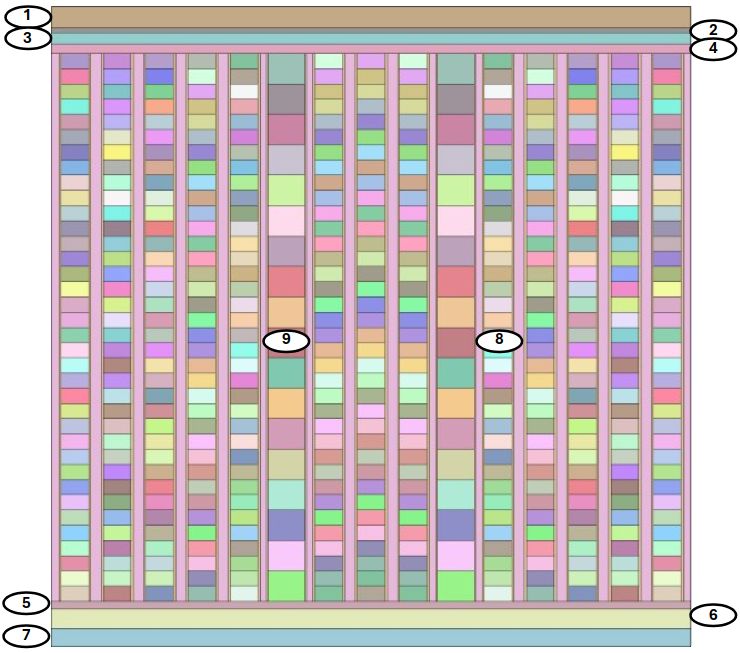
\includegraphics[width=0.65\linewidth]{figs/TMI_xz_plot.png}
    \caption{Axial cross-section of the TMI-1 fuel assembly Serpent geometry showing subdivided depletion zones. Structural components are labeled; axes are not to scale.}
    \label{fig:tmi_geometry}
\end{figure}

\begin{table}[H]
\centering
\caption{Labeled components of the TMI-1 fuel assembly geometry shown in Figure~\ref{fig:tmi_geometry}. Dimension $t$ denotes axial thickness; $d$, $L$, and $p$ denote diameter, active length, and rod pitch, respectively.}
\label{tab:figure_labels}
\renewcommand{\arraystretch}{1.4}
\begin{tabular}{c l l l}
\toprule
\textbf{Label} & \textbf{Component} & \textbf{Dimensions [cm]} & \textbf{Material} \\
\midrule
\ovalbox{1} & Upper Plenum   & $t = 14.14$ & SS-304 / borated water \\
\ovalbox{2} & Upper Flange   & $t = 3.18$  & SS-304 / borated water \\
\ovalbox{3} & Upper Grid     & $t = 7.62$  & SS-304 / borated water \\
\ovalbox{4} & Upper Pad      & $t = 5.08$  & SS-304 / borated water \\
\ovalbox{5} & Lower Pad      & $t = 5.08$  & SS-304 / borated water \\
\ovalbox{6} & Lower Grid     & $t = 12.70$ & SS-304 / borated water \\
\ovalbox{7} & Lower Plate    & $t = 12.22$ & SS-304 / borated water \\
\midrule
\ovalbox{8} & Fuel Rod &
\parbox[t]{3.4cm}{%
  $d_\text{pellet}   = 0.935$\\
  $d_\text{clad,in}  = 0.958$\\
  $d_\text{clad,out} = 1.092$\\
  $L_\text{active}   = 360.17$\\
  $p = 1.4427$
} &
\parbox[t]{3.4cm}{%
  UO\textsubscript{2} (4.0\,wt\%)\\
  Zircaloy-4 cladding\\
  He fill gas
} \\[1.8cm]
\ovalbox{9} & \parbox[t]{2.5cm}{Burnable\\Poison Rod} &
\parbox[t]{3.4cm}{%
  $d_\text{in}  = 1.265$\\
  $d_\text{out} = 1.346$\\
  $L_\text{active} = 360.17$
} &
\parbox[t]{3.4cm}{%
  Al\textsubscript{2}O\textsubscript{3}--B\textsubscript{4}C\\
  Zircaloy-4 cladding
} \\[1.0cm]
\bottomrule
\end{tabular}
\end{table}

% ============================================================
\subsubsection{Operating History and Depletion Solver Stability}
% ============================================================

Burnup simulations followed the irradiation history of Assembly NJ05YU as documented in \cite{Wolf2000AnalysisReport}, comprising: a 666-day first cycle with control rods fully inserted, a 36-day shutdown period, and a 692-day second cycle with control rods fully withdrawn. A constant assembly fission power of 14.508\,MW was maintained throughout all operating periods. The assembly-averaged discharge burnup is approximately 30\,GWd/MTU.

Two independent simulations of the operating history were performed, each using different numerical solver configurations — specifically, different depletion algorithms (CRAM-16 vs.\ a substep method) and timestep discretizations — in order to assess the sensitivity of isotopic predictions to solver parameters. As shown in Figure~\ref{fig:tmi-stability}, solver selection has a non-trivial effect on the predicted nuclide evolution, particularly for short-lived intermediaries and actinide chains that are sensitive to numerical stiffness. The stable configuration, characterized by finer substep divisions and higher-order CRAM, was adopted for all subsequent material generation.

\begin{figure}[H]
    \centering
    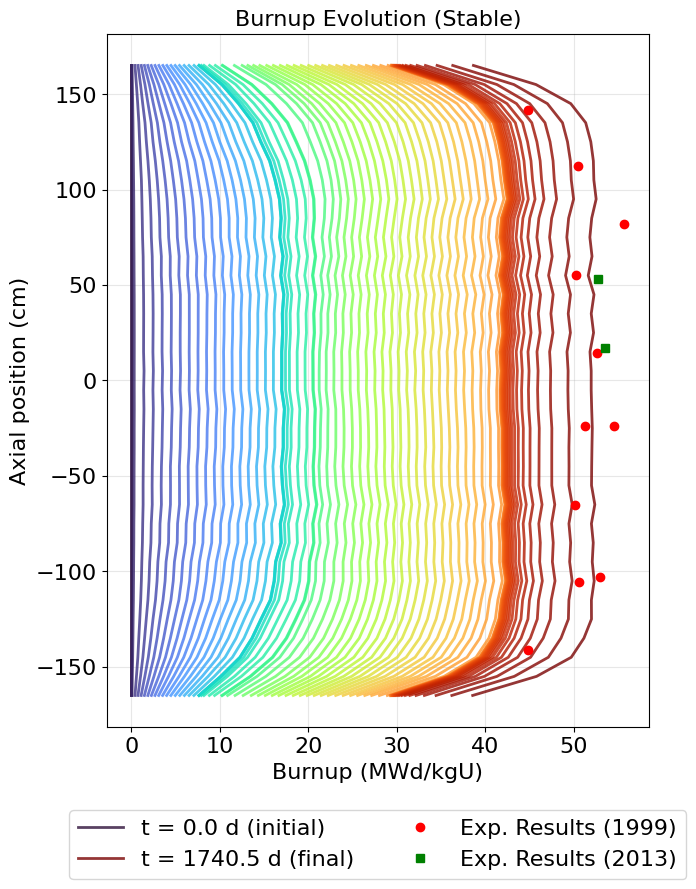
\includegraphics[width=0.48\linewidth]{figs/TMI_evol_stable.png}
    \hfill
    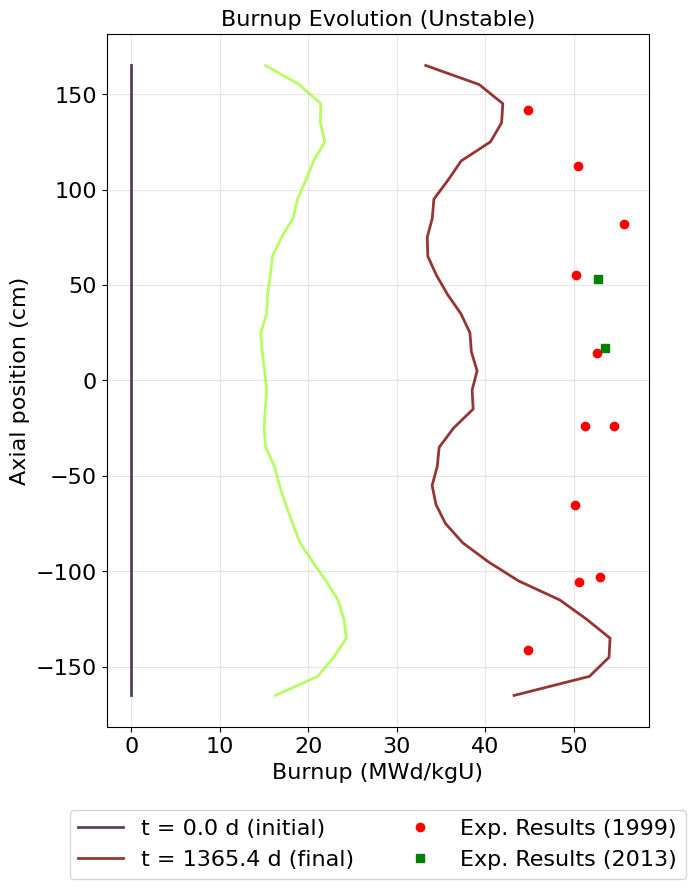
\includegraphics[width=0.48\linewidth]{figs/TMI_evol_unstable.png}
    \caption{Comparison of nuclide evolution computed with a numerically stable solver configuration (left) and an unstable configuration (right). Differences in predicted isotopic inventories highlight the sensitivity of burnup calculations to depletion timestep size and solver order, motivating careful solver selection prior to material extraction.}
    \label{fig:tmi-stability}
\end{figure}

% ============================================================
\subsubsection{Isotopic Validation Against Experimental Data}
% ============================================================

Spatial isotopic distributions predicted by the Serpent model were validated against radiochemical assay measurements of Assembly NJ05YU, originally reported in 1999 and subsequently re-evaluated in 2013 using updated nuclear data libraries \cite{Wolf2000AnalysisReport}. Validation focused on two key isotopes of interest: $^{235}$U, which serves as the primary fissile driver during irradiation, and $^{239}$Pu, whose in-situ production and consumption governs the breeding performance of the LBR concept.

The predicted axial distribution of $^{235}$U concentration is shown in Figure~\ref{fig:U235_evol_tmi} alongside experimental data at each reported irradiation stage. Simulation results fall within the $2\sigma$ uncertainty bounds of the measured data across the full active length, providing high confidence in the depletion model's treatment of $^{235}$U burnout.

\begin{figure}[H]
    \centering
    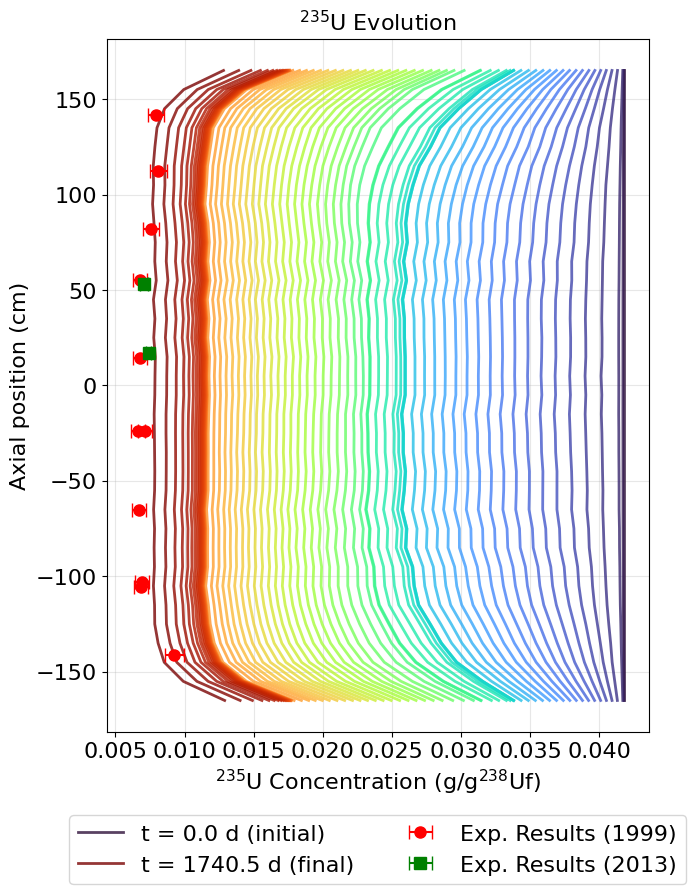
\includegraphics[width=0.65\linewidth]{U235_evol_tmi.png}
    \caption{Axial distribution of $^{235}$U concentration from initial loading through discharge, compared against radiochemical assay data. Simulation results (solid lines) fall within the $2\sigma$ experimental uncertainty bounds (shaded) at all irradiation stages, confirming the accuracy of the depletion model for the primary fissile species.}
    \label{fig:U235_evol_tmi}
\end{figure}

The predicted axial distribution of $^{239}$Pu is shown in Figure~\ref{fig:Pu239_evol_tmi}. Simulated results deviate considerably from the 1999 experimental dataset, but align closely with the 2013 re-evaluation, which incorporated revised cross-section libraries and updated decay data. This discrepancy is attributed to improvements in the nuclear data used for Pu production and capture reactions rather than deficiencies in the transport model itself. The agreement with the 2013 dataset provides confidence that the current simulation correctly captures plutonium buildup — a quantity of central importance to LBR breeding performance.

\begin{figure}[H]
    \centering
    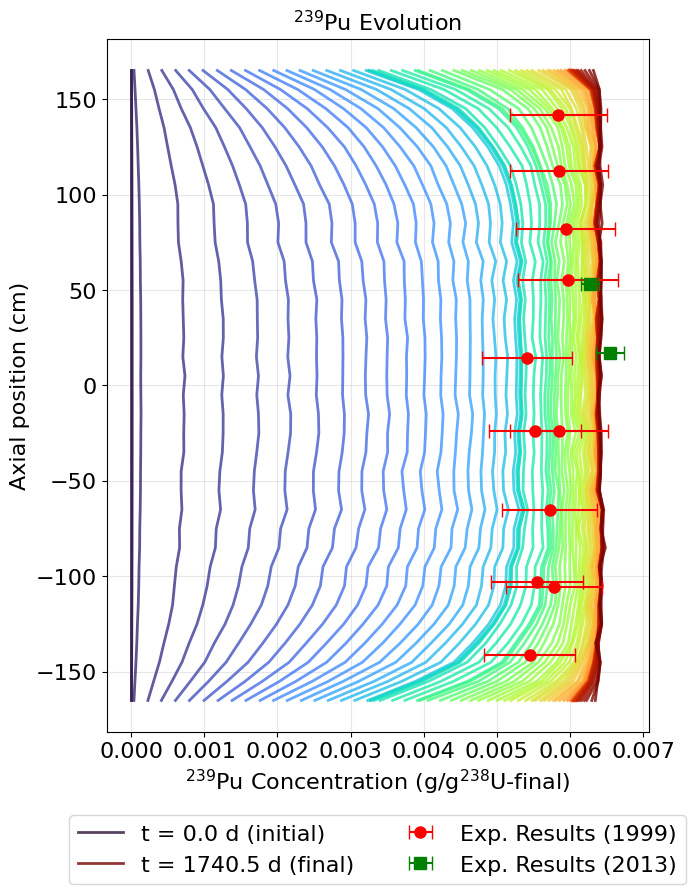
\includegraphics[width=0.65\linewidth]{Pu239_evol_tmi.png}
    \caption{Axial distribution of $^{239}$Pu concentration from initial loading through discharge, compared against the 1999 experimental assay and the 2013 re-evaluation. The improved agreement with the 2013 dataset is attributed to updated nuclear data libraries rather than model deficiencies, and provides confidence in predicted plutonium breeding behavior.}
    \label{fig:Pu239_evol_tmi}
\end{figure}

Taken together, the $^{235}$U and $^{239}$Pu validation results demonstrate that the TMI-1 depletion model accurately reproduces the isotopic composition of spent LWR fuel. The validated material definitions are subsequently transferred to the LBR lattice model via Serpent's binary restart file mechanism, eliminating interpolation error and preserving the full nuclide inventory for each axial depletion zone.

% ============================================================
\subsection{Moderator and Lattice Pitch Selection}
% ============================================================

The choice of moderator material and lattice pitch exerts the strongest influence on the neutron energy spectrum, initial reactivity, and the balance between fission and breeding reactions. Following the approach used in the preliminary 0-D scoping studies, a parametric sweep was conducted over a range of lattice pitches for each candidate moderator material. Candidate moderators considered in this study include light water (H$_2$O), heavy water (D$_2$O), and graphite. Spent fuel material definitions were transferred directly from the validated TMI-1 model via binary restart file, without fuel shuffling, ensuring that the lattice-level neutronics are evaluated using a physically consistent starting composition.

Two figures of merit (FOM) were used to guide pitch selection:
\begin{enumerate}
    \item \textbf{Initial excess reactivity} ($k_\infty - 1$): a measure of how much reactivity margin is available at the start of the critical cycle, which sets an upper bound on achievable cycle length.
    \item \textbf{Burn-to-breed ratio of $^{239}$Pu}: defined as the ratio of $^{239}$Pu consumed by fission to $^{239}$Pu produced by $^{238}$U capture, which quantifies the degree to which the assembly operates as a breeder versus a burner.
\end{enumerate}

The dependence of each FOM on lattice pitch and moderator selection is shown in Figures~\ref{fig:keff_sweep} and~\ref{fig:b2b_sweep}, respectively.

\begin{figure}[H]
    \centering
    \includegraphics[width=0.5\linewidth]{figs/absKeffLBR.png}
    \caption{Infinite multiplication factor $k_\infty$ as a function of lattice pitch for each candidate moderator material. Each curve reflects a constant spent fuel composition transferred from the TMI-1 benchmark model.}
    \label{fig:keff_sweep}
\end{figure}

\begin{figure}[H]
    \centering
    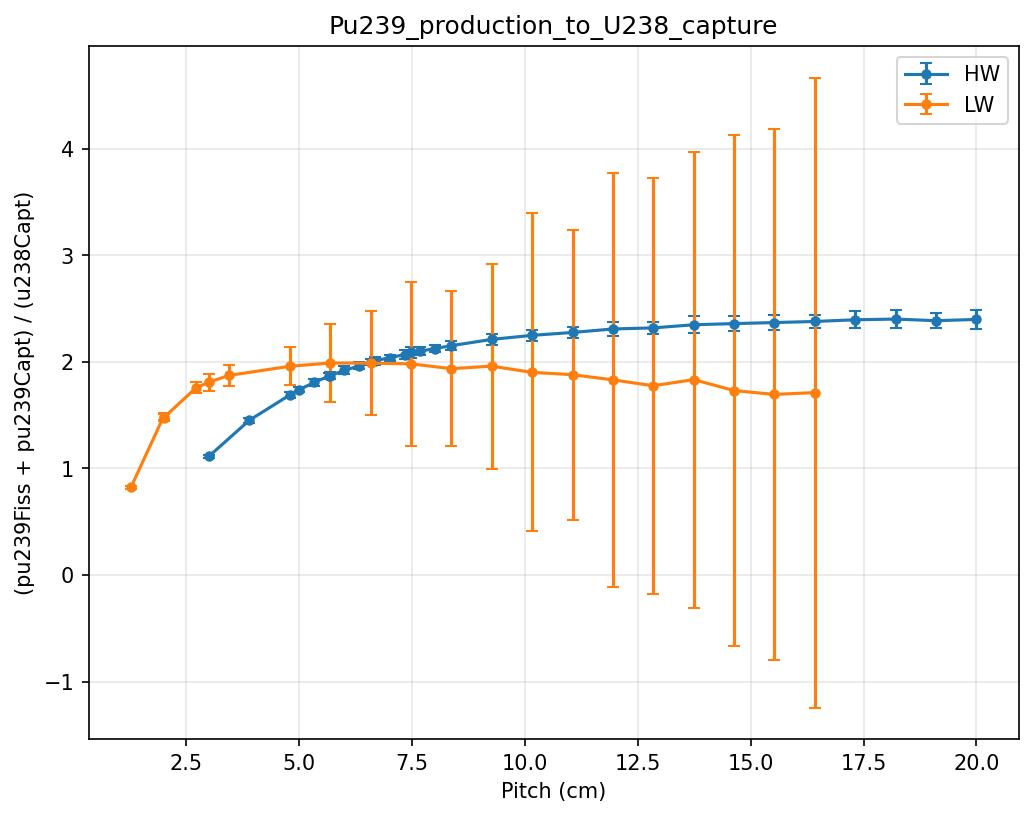
\includegraphics[width=0.5\linewidth]{figs/burnToBreedLBR.png}
    \caption{Burn-to-breed ratio of $^{239}$Pu as a function of lattice pitch for each candidate moderator. Values below unity indicate net plutonium production (breeding mode); values above unity indicate net consumption (burning mode).}
    \label{fig:b2b_sweep}
\end{figure}

Based on the results of the pitch sweep, a lattice pitch of 6\,cm with heavy water moderation was selected as the reference design point. This combination yields a sufficiently positive initial reactivity to support a meaningful critical cycle length while maintaining a burn-to-breed ratio below unity — indicating net in-situ plutonium production. This conclusion is consistent with the findings from the preliminary infinite-lattice scoping studies, providing cross-validation of the methodology across two levels of geometric fidelity.

% ============================================================
\subsection{Design Iteration}
% ============================================================

Examination of Figures~\ref{fig:U235_evol_tmi} and~\ref{fig:Pu239_evol_tmi} reveals a characteristic feature of PWR spent fuel: the upper and lower $\sim$50\,cm of each fuel rod retain a notably higher inventory of fissile material ($^{235}$U and $^{239}$Pu) relative to the axial midplane, due to flux depression by the adjacent structural hardware and control rod shadowing effects during the first irradiation cycle. In the baseline LBR configuration, these under-depleted end regions represent an underutilized fissile resource. Design iteration was therefore aimed at redistributing fission power toward the rod extremities to more efficiently exploit this inventory.

Design performance was assessed using two figures of merit evaluated at the end of the critical cycle:

\begin{enumerate}
    \item \textbf{Critical cycle length}: the duration over which $k_\text{eff} \geq 1$ is maintained, serving as a proxy for energy extraction and economic viability.
    \item \textbf{Coefficient of variation (CV) of fissile isotope distribution}: a dimensionless measure of axial uniformity in the fissile inventory at end-of-life, defined as:
\end{enumerate}

\begin{equation}
    \text{CV} = \frac{s}{\bar{w}} \times 100\%
    \label{eq:cv}
\end{equation}

\noindent where the sample mean $\bar{w}$ and standard deviation $s$ of the axial fissile weight fraction distribution are:

\begin{equation}
    \bar{w} = \frac{1}{N} \sum_{i=1}^{N} w_i, \qquad
    s = \sqrt{\frac{1}{N-1} \sum_{i=1}^{N} \left(w_i - \bar{w}\right)^2}
    \label{eq:cv_components}
\end{equation}

\noindent Here, $N$ is the number of equally sized axial depletion nodes, and $w_i$ is the total fissile weight percent (summed over $^{235}$U and $^{239}$Pu) at node $i$. A lower CV at end-of-life indicates a more axially uniform depletion profile, which is beneficial from both neutronics and fuel management perspectives, as it implies more complete utilization of the available fissile inventory and reduced peak-to-average power factors. Note that this metric is valid only for a uniform axial discretization in which each node $w_i$ represents an equal-length segment of the active fuel column.

Four design variants were evaluated, each representing a different strategy for redistributing fission power toward the rod extremities:

\paragraph{Baseline (Spent Fuel As-Is).}
In this configuration, the LBR assembly is loaded exclusively with spent PWR fuel rods in their as-discharged condition, with no additional devices or structural modifications. This case serves as the reference against which all modified designs are compared.

\paragraph{Beryllium End Reflectors.}
In this design, each fuel rod is fitted with beryllium ($^9$Be) axial reflector plugs in the upper and lower 70\,cm of the active zone, as illustrated in Figure~\ref{fig:be_caps_sketch}. Beryllium is an effective fast-neutron reflector and moderator due to its low neutron capture cross section and significant scattering cross section, and it is a neutron multiplier via the $^9$Be$(n,2n)$ reaction. The intent is to reflect neutrons that would otherwise stream axially out of the assembly back into the fissile end regions, thereby increasing the local thermal flux and enhancing fission rates in the less-depleted rod extremities.

\paragraph{Fresh Fuel Rods.}
In this design, every alternate lattice position is occupied by a fresh fuel rod. These rods have a graded enrichment profile: the central region (coinciding with the high-burnup zone of adjacent spent rods) is loaded with 5\,wt.\%\,UO$_2$, while the end regions are loaded with 10\,wt.\%\,UO$_2$ to compensate for the lower reactivity in the axial periphery and to promote peaked fission power at the rod extremities. This design introduces fresh fissile material as an active power-shaping tool.

\paragraph{Power Inverter Device.}
In this design, every alternate lattice position is occupied by a novel component designated the \textit{Power Inverter}. In the reference Power Inverter configuration, the upper and lower 70\,cm of each device contain 5\,wt.\%\,UO$_2$ fuel pins, while the central region is occupied by cerium dioxide (CeO$_2$, ceria) pins — all enclosed within a shared Zircaloy-4 cladding tube. The Power Inverter is designed to invert the axial power profile relative to the baseline: fission is concentrated in the end regions (co-located with the under-depleted extremities of the surrounding spent rods), while the central region contributes negligible fission power.

Ceria was selected as the central inert fill material for several reasons: (i) it is largely transparent to thermal neutrons due to its low absorption cross section, allowing the axial neutron flux to diffuse into the end fuel regions without being parasitically absorbed; (ii) it is chemically inert and thermally stable at LWR operating temperatures; and (iii) it shares closely matched thermo-mechanical properties with UO$_2$ — including crystal structure (fluorite), thermal conductivity, and coefficient of thermal expansion — which mitigates stress concentration and material compatibility concerns at the CeO$_2$/UO$_2$ interface.

The performance of each design variant against the two figures of merit is discussed in Section~\ref{sec:results}. % <-- update cross-ref as needed


\begin{figure}[H]
    \centering
    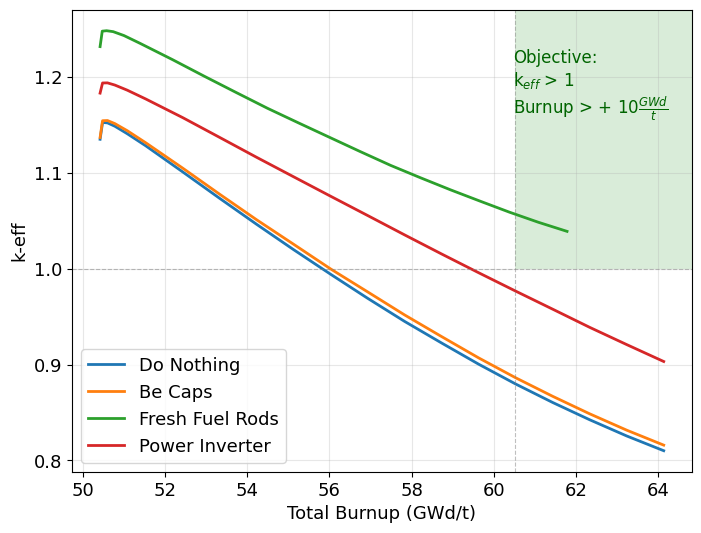
\includegraphics[width=0.75\linewidth]{figs/4-designs-keff.png}
    \caption{Enter Caption}
    \label{fig:placeholder}
\end{figure}

\begin{figure}[H]
    \centering
    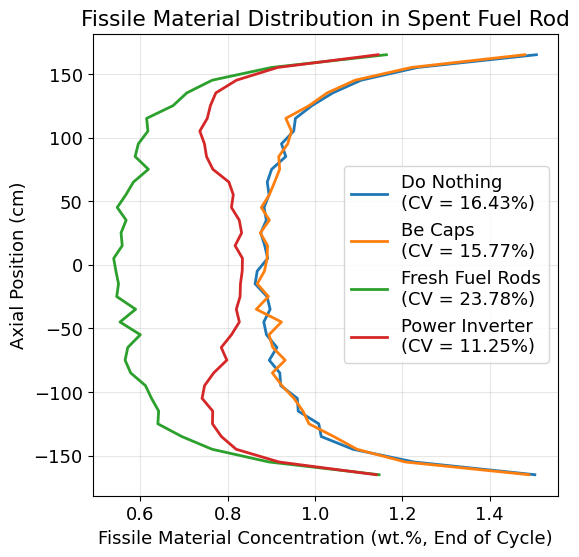
\includegraphics[width=0.75\linewidth]{figs/4-designs-fiss-dist.png}
    \caption{Enter Caption}
    \label{fig:placeholder}
\end{figure}

\newpage

\begin{figure}[H]
    \centering
    \begin{subfigure}[t]{0.48\linewidth}
        \centering
        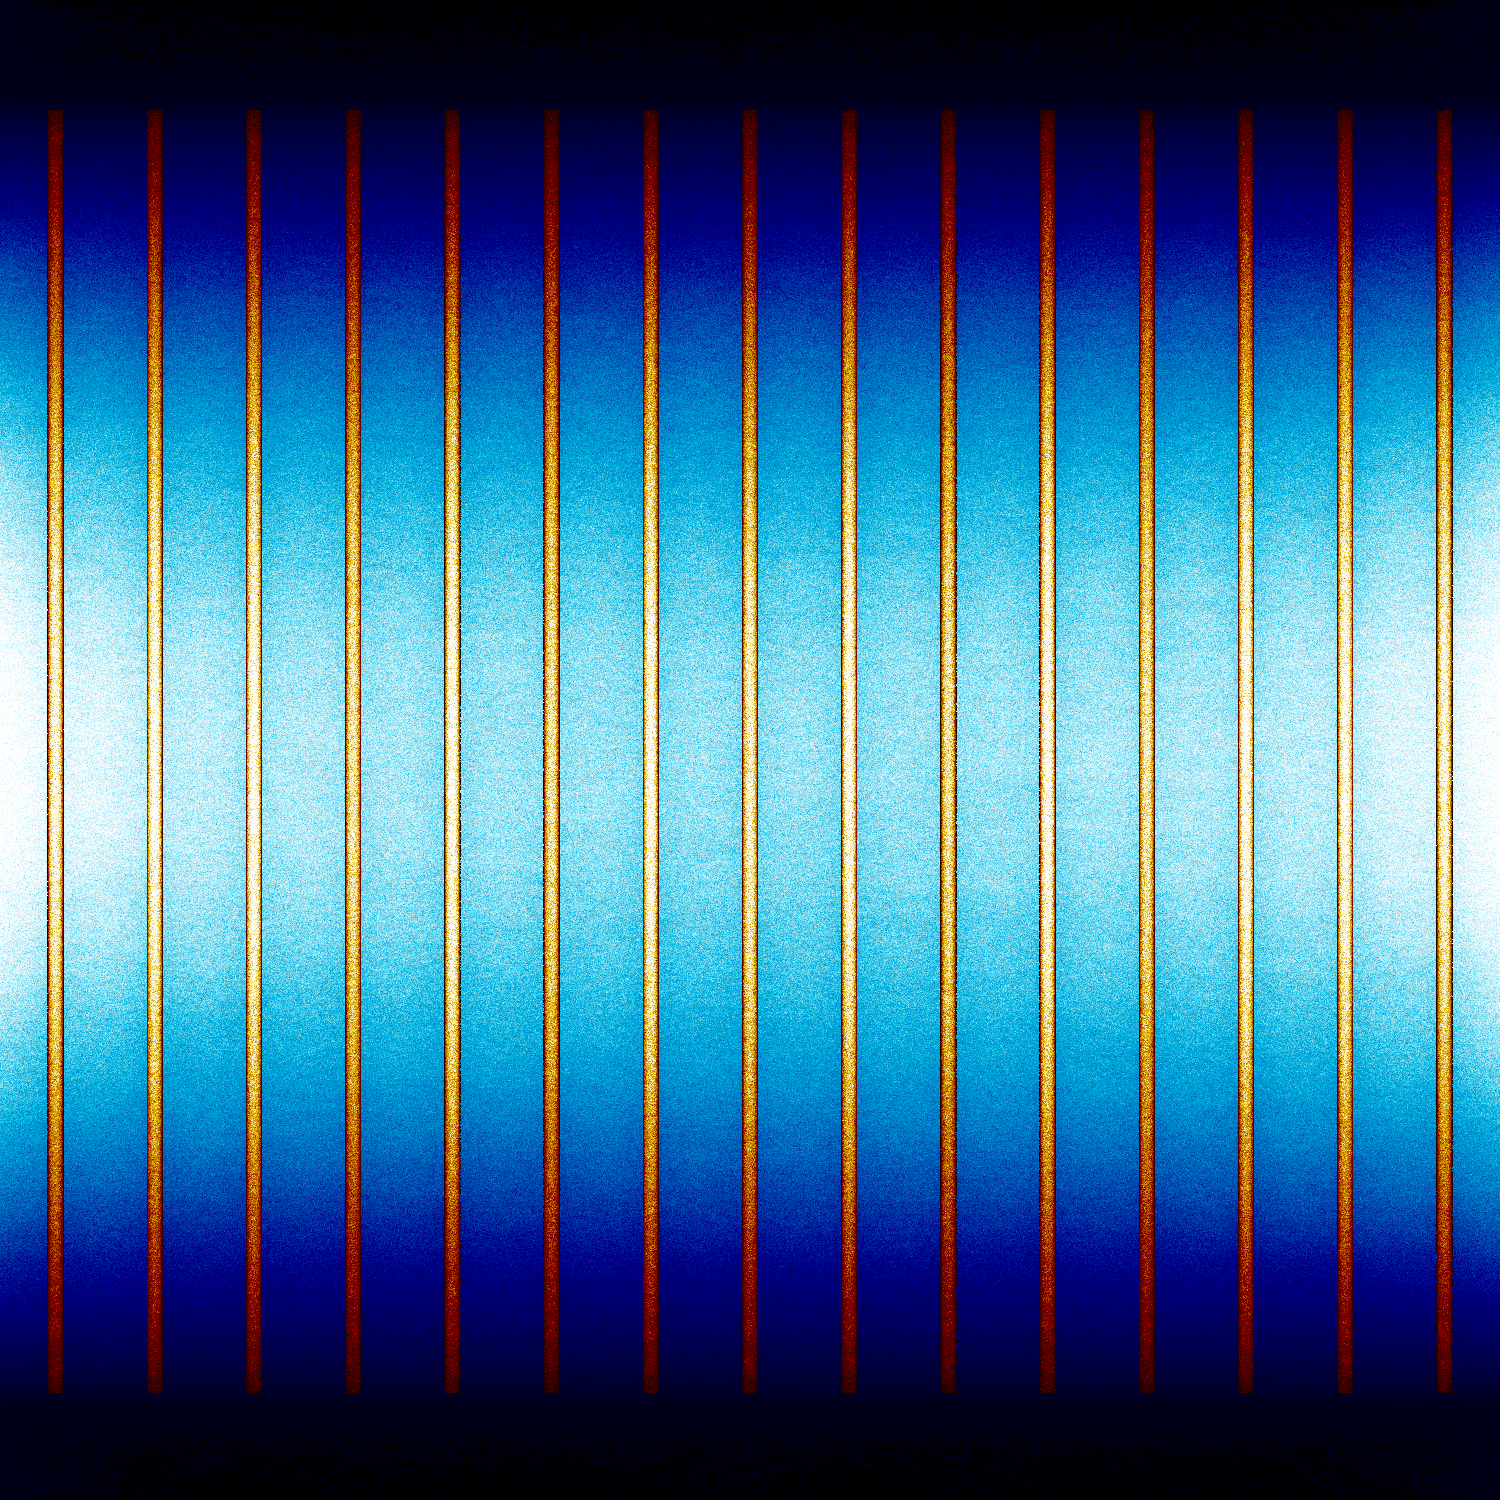
\includegraphics[width=\linewidth]{figs/powerdist-donothing.png}
        \caption{Baseline}
    \end{subfigure}
    \hfill
    \begin{subfigure}[t]{0.48\linewidth}
        \centering
        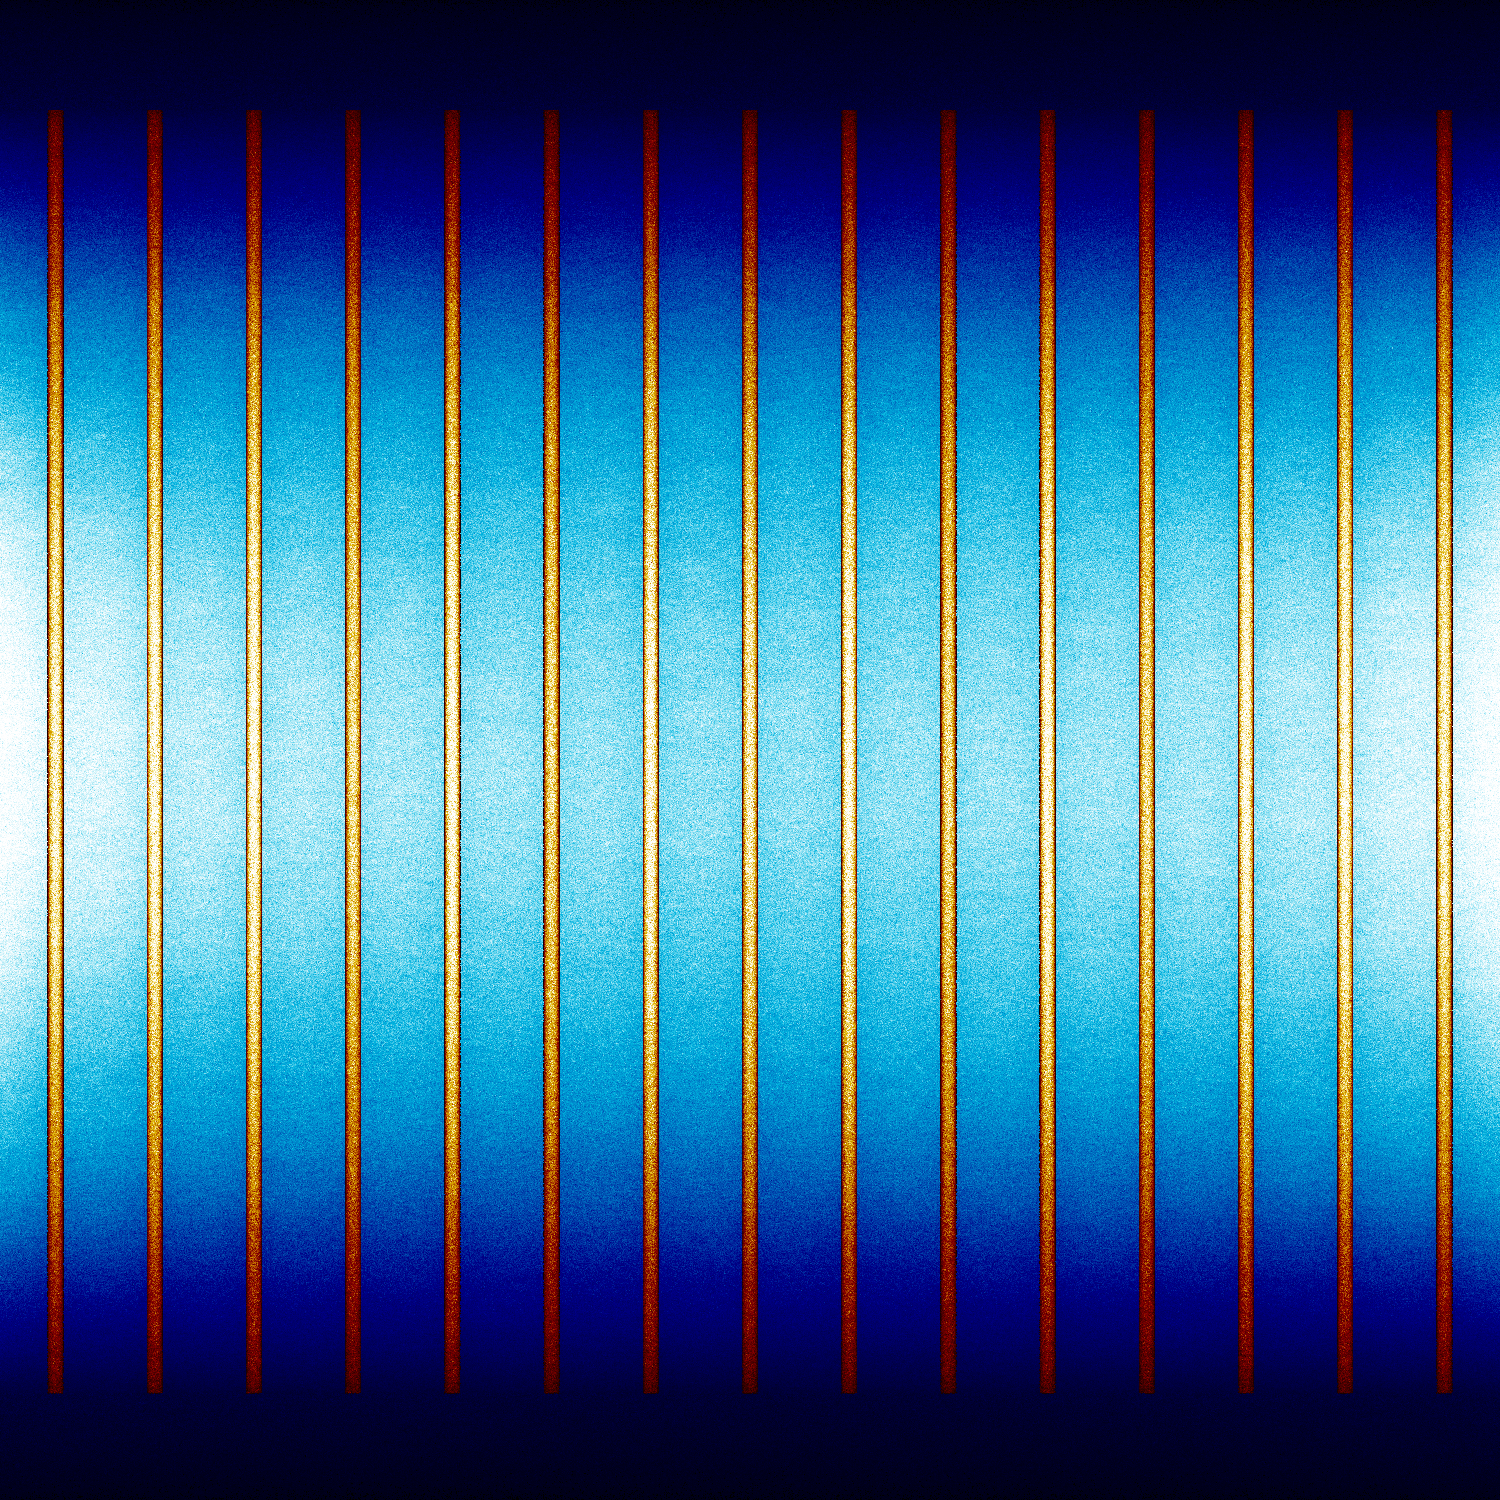
\includegraphics[width=\linewidth]{figs/powerdist-becaps.png}
        \caption{Beryllium End Reflectors}
    \end{subfigure}

    \medskip

    \begin{subfigure}[t]{0.48\linewidth}
        \centering
        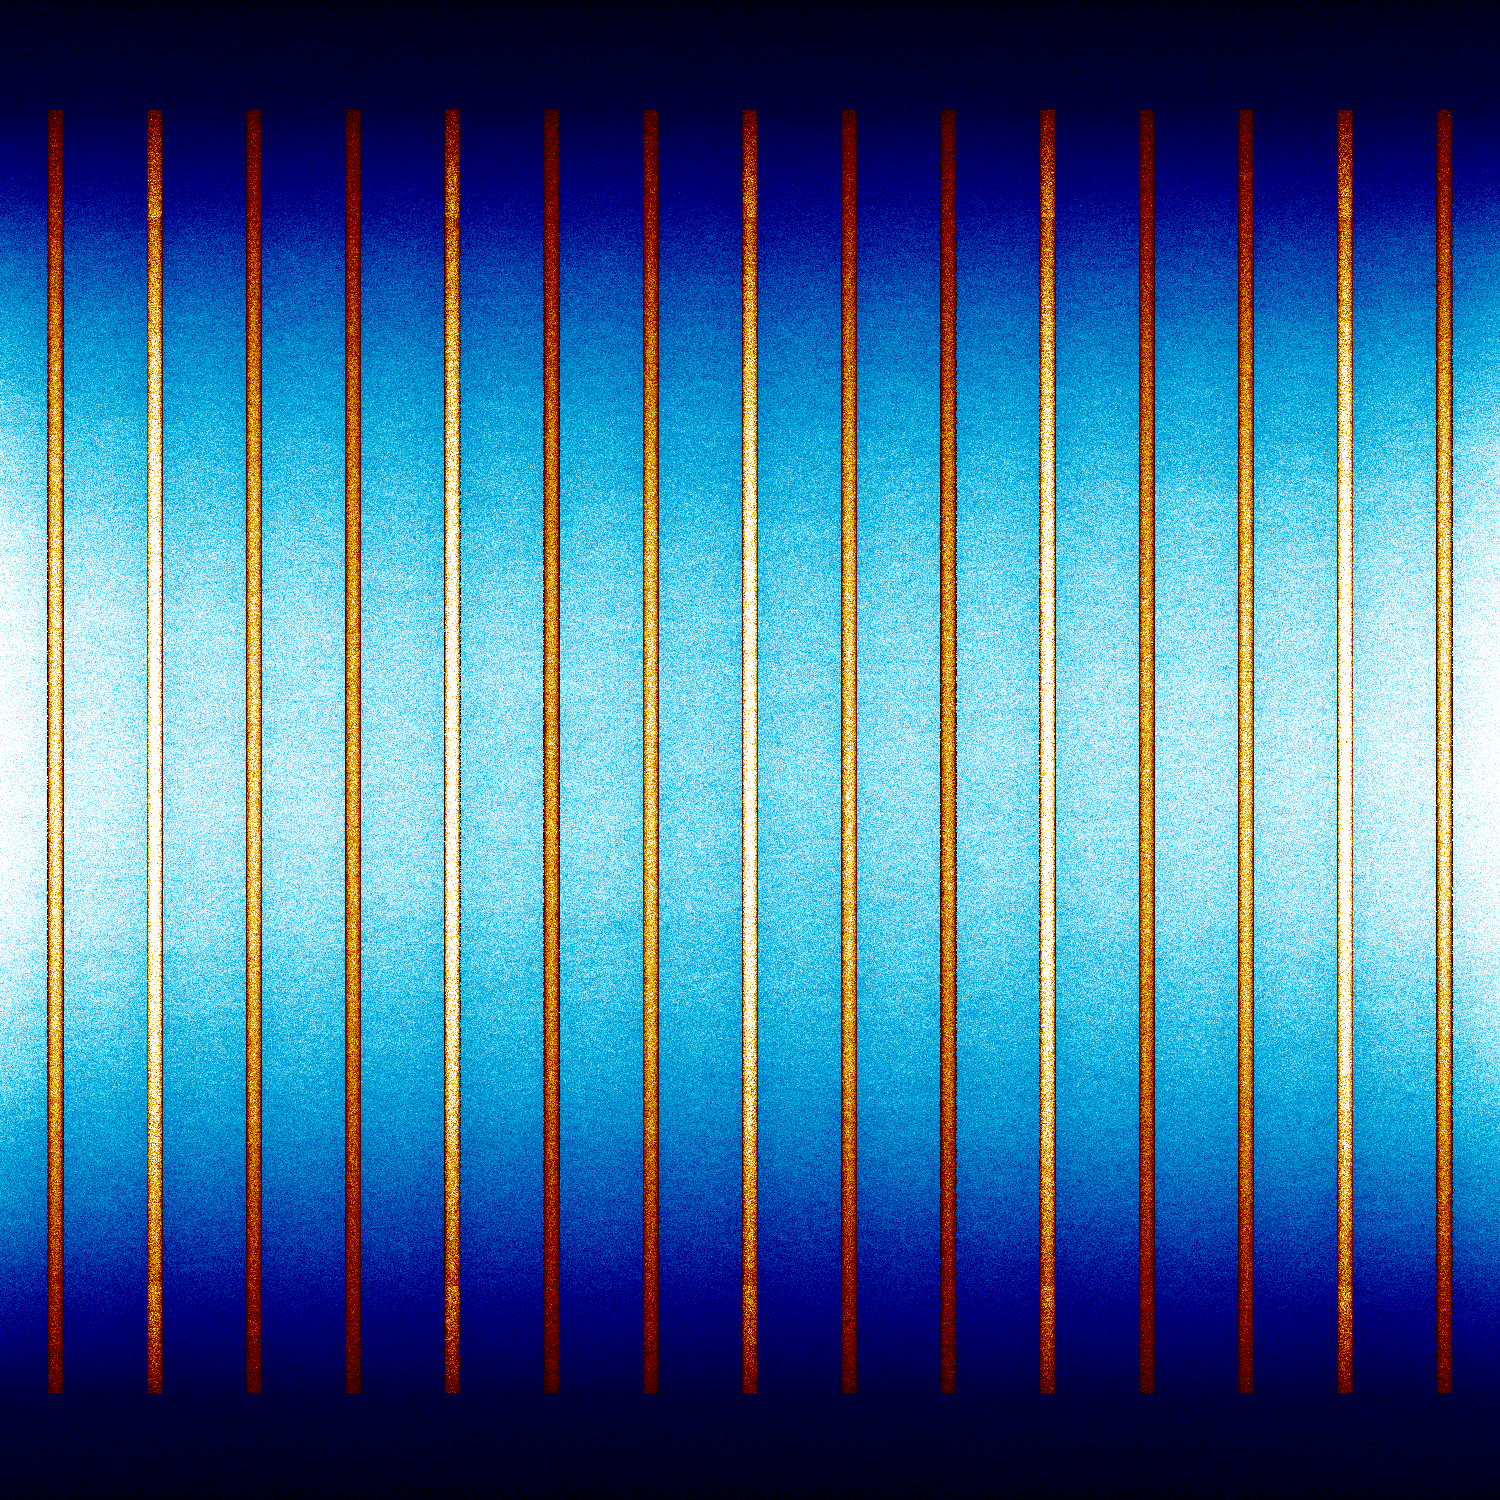
\includegraphics[width=\linewidth]{figs/powerdist-freshrods.png}
        \caption{Fresh Fuel Rods}
    \end{subfigure}
    \hfill
    \begin{subfigure}[t]{0.48\linewidth}
        \centering
        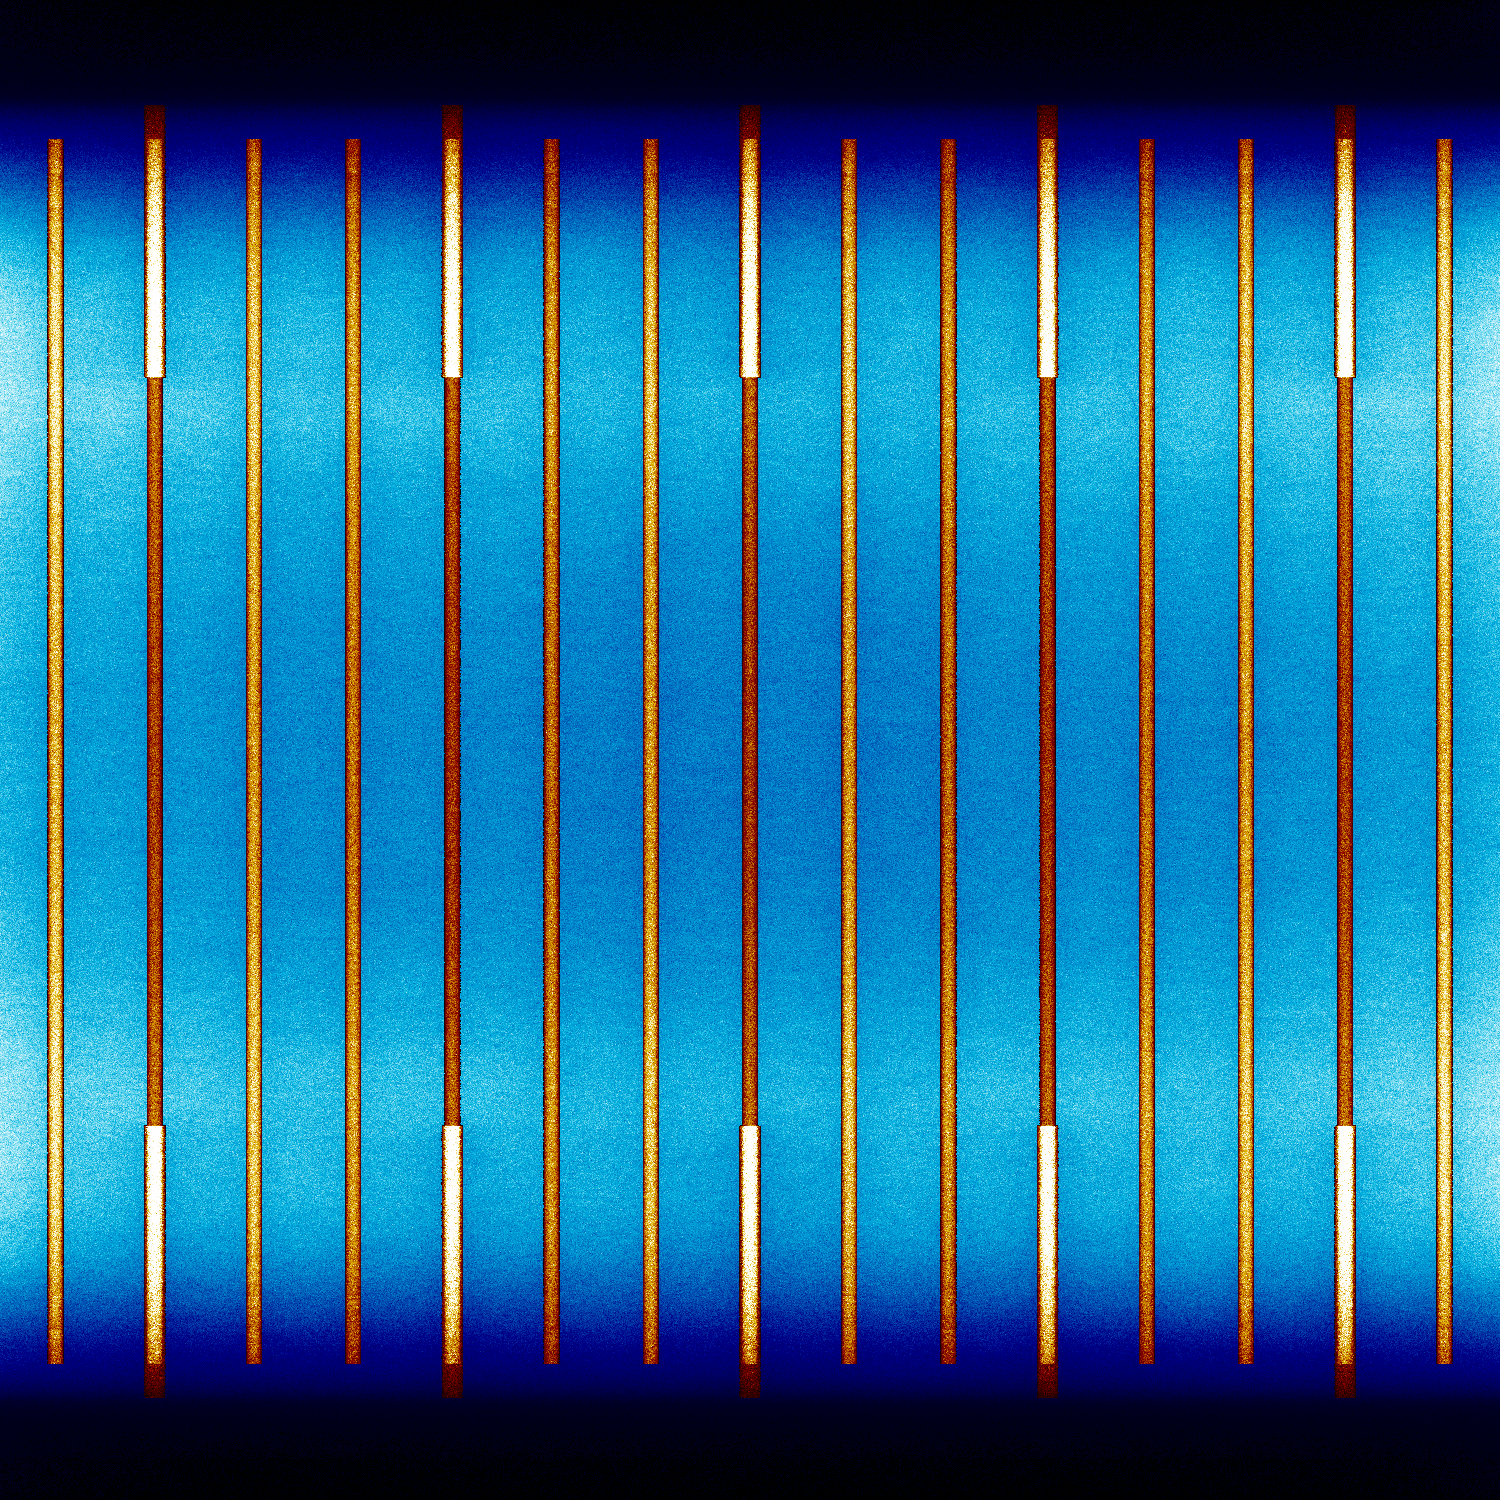
\includegraphics[width=\linewidth]{figs/powerdist-powerinverter.png}
        \caption{Power Inverter Device}
    \end{subfigure}

    \caption{Power distribution profiles under each mitigation strategy.}
\end{figure}

\usepackage{makecell} % in preamble

\begin{table}[H]
    \centering
    \renewcommand{\arraystretch}{1.8}
    \begin{tabular}{>{\bfseries\raggedright\arraybackslash}m{3.8cm} 
                    >{\centering\arraybackslash}m{1.2cm} 
                    >{\centering\arraybackslash}m{1.8cm} 
                    >{\centering\arraybackslash}m{1.5cm} 
                    >{\centering\arraybackslash}m{1.8cm} 
                    >{\centering\arraybackslash}m{1.5cm}}
    \toprule
    \textbf{Criteria} & \textbf{Weight} & \textbf{Do Nothing} & \textbf{Be Caps} & \textbf{Fresh Fuel} & \textbf{Power Inv.} \\
    \midrule
    Critical Cycle Length        & 0.4 & 1 & 1 & 4 & 3 \\
    Reliance on Spent Fuel       & 0.3 & 4 & 3 & 1 & 2 \\
    Utilization of lesser-depleted regions & 0.3 & 2 & 3 & 1 & 4 \\
    \midrule
    \textbf{Total} & \textbf{1.0} & \textbf{2.2} & \textbf{2.2} & \textbf{2.2} & \textbf{3.0} \\
    \bottomrule
    \end{tabular}
    \caption{Weighted decision matrix for mitigation strategies.}
\end{table}

Based upon the results of the 4 designs, it is justified to continue iterating upon the power inverter design. Because each simulation requires \>24 hours of wall time, a simplified model of the assembly was made using periodic boundary conditions -- as shown in Figure \ref{}. Although there are large discrepancies between the simplified model and higher-fidelity results, the simplified model completes the burnup simulation in \< 1 hour and provides general insight allowing for a large parametric sweep.

\begin{figure}[H]
    \centering
    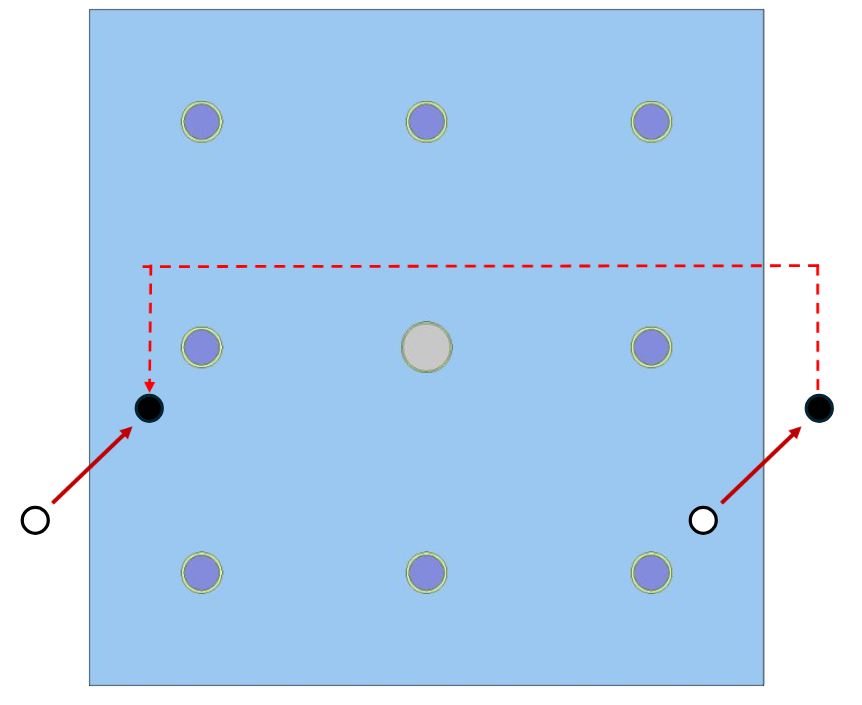
\includegraphics[width=0.5\linewidth]{figs/simplified-lbr.png}
    \caption{Enter Caption}
    \label{fig:placeholder}
\end{figure}

The parametric sweep was conducted for the length and enrichment of the fuel regions of the Power Inverter. Results for the CV and critical cycle length are shown in Figures \ref{} and \ref{} respectively.

\begin{figure}[H]
    \centering
    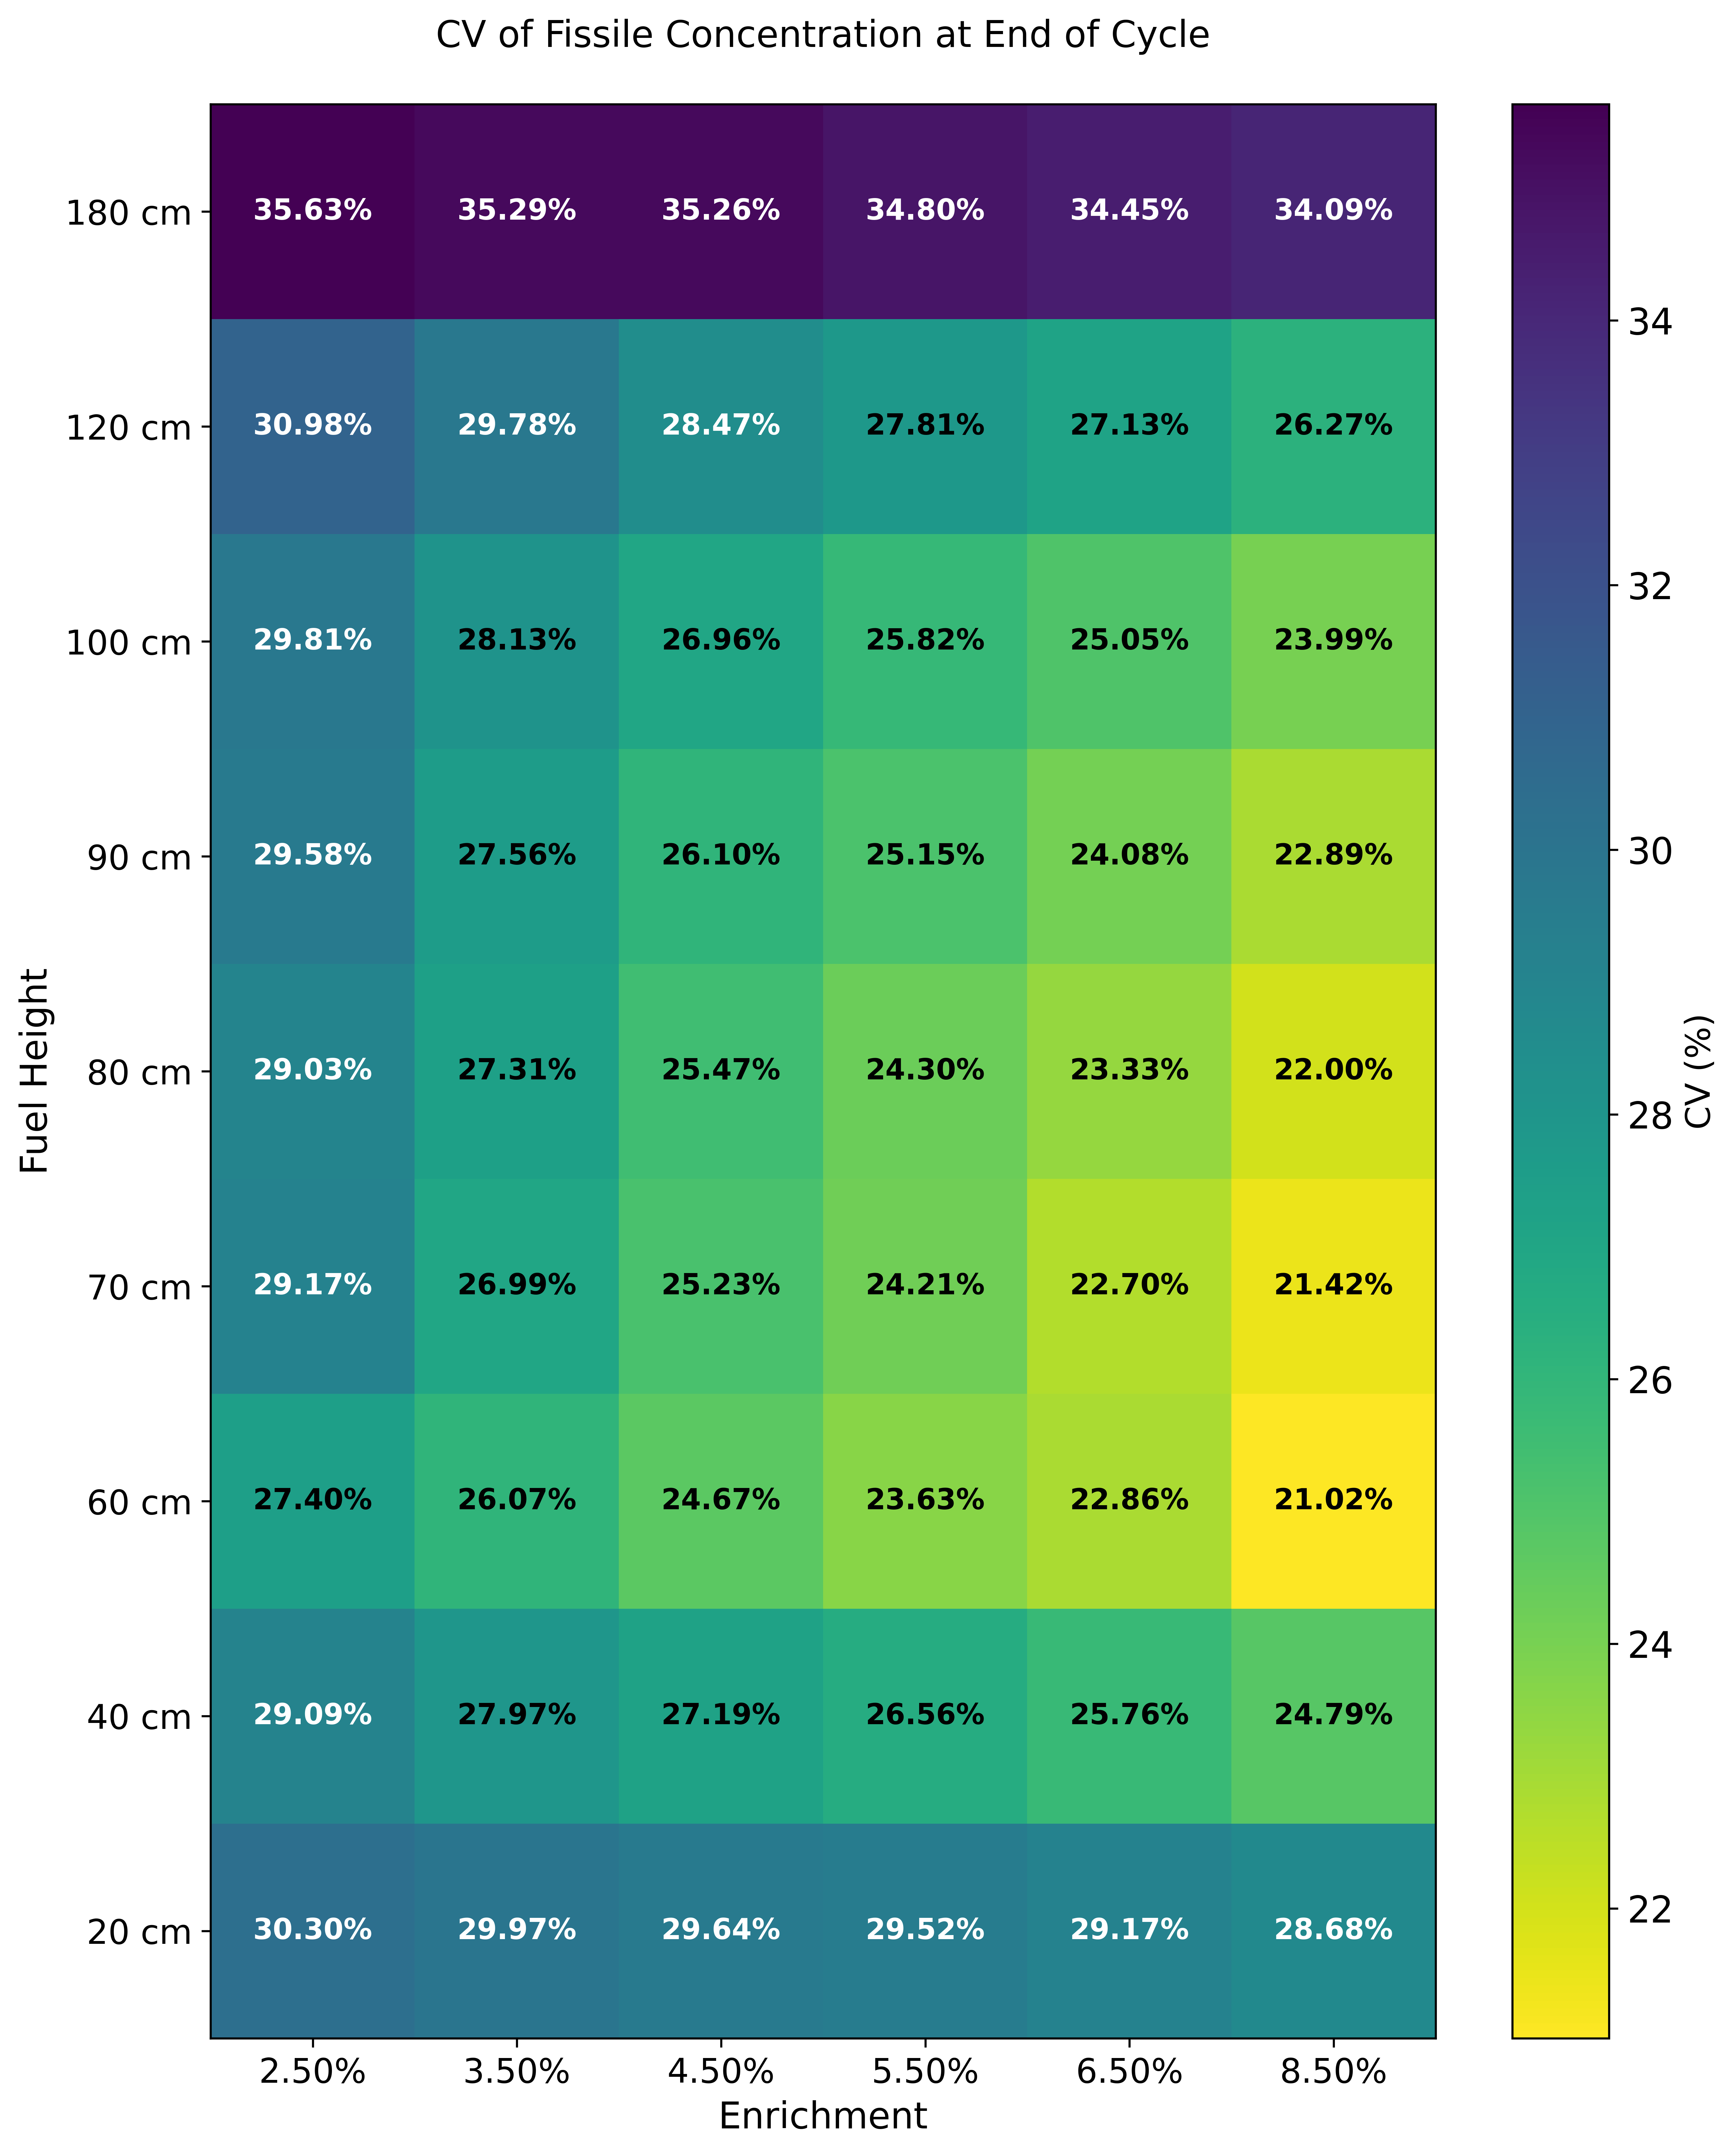
\includegraphics[width=0.8\linewidth]{figs/power-inverter-sweep-cv.png}
    \caption{Coefficient of variance results from power inverter parametric sweep. The length of fuel regions varied in height and enrichment. The study reveals that optimal length is between 60 and 80 cm}
    \label{fig:placeholder}
\end{figure}

\begin{figure}[H]
    \centering
    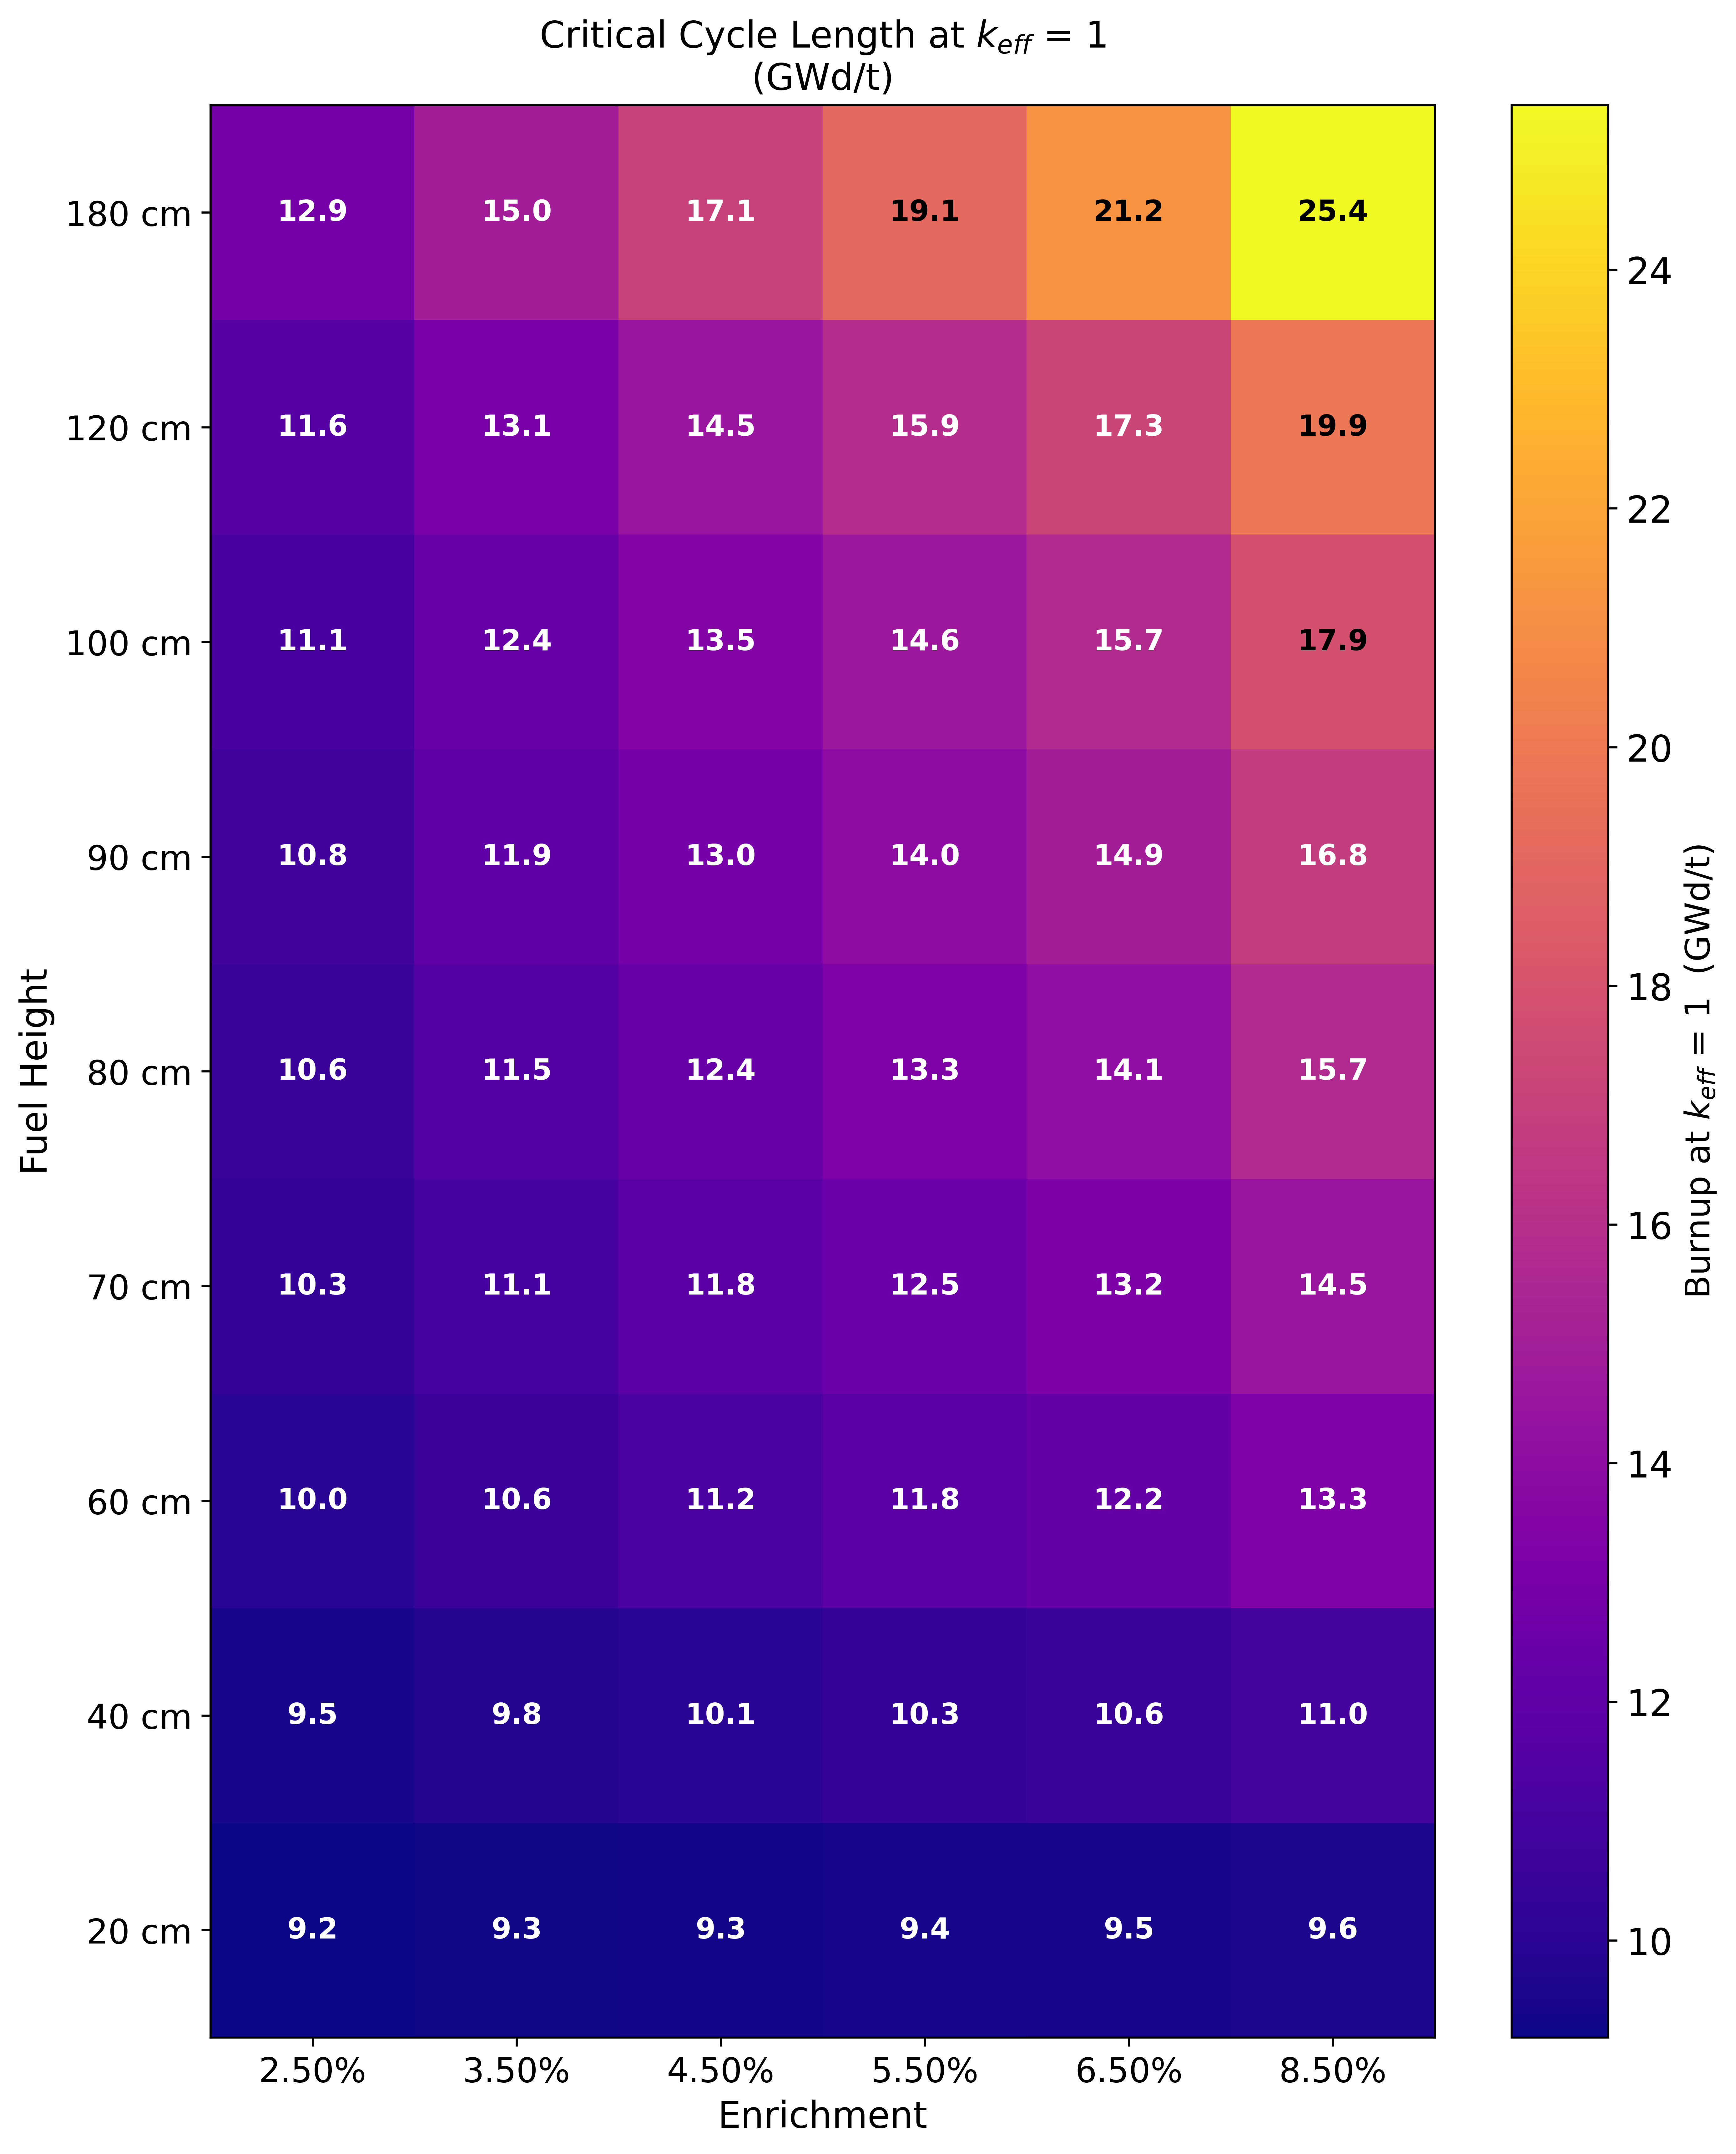
\includegraphics[width=0.8\linewidth]{figs/power-inverter-sweep-length.png}
    \caption{Enter Caption}
    \label{fig:placeholder}
\end{figure}